% Bachelor's Thesis Template: Biological Learning Models in ML
% No title page or abstract; front matter of 4 pages (2 blank, acknowledgements, blank)
% Page numbering starts after front matter.

\documentclass[a4paper,12pt]{report}
\usepackage[paperwidth=21cm,paperheight=29.7cm,left=2.5cm,right=2.5cm,top=2.5cm,bottom=2.5cm]{geometry}
\usepackage{setspace}
\usepackage{tocloft}
\usepackage{parskip}
\usepackage{graphicx} % For including images
\usepackage{xcolor}
\usepackage{cite}
\usepackage{amssymb} % For \mathbb
\usepackage{amsmath} % For \operatorname
\usepackage[hidelinks]{hyperref}
\usepackage{tikz}
\usepackage{algorithm}
\usepackage{algpseudocode}
\usepackage{caption}

\usetikzlibrary{backgrounds, shapes.geometric, positioning, fit, arrows.meta}


\setlength{\cftbeforechapskip}{1em}
\setlength{\cftbeforesecskip}{0.5em}

\hypersetup{
  colorlinks=true,
  linkcolor=black,
  filecolor=black,      
  urlcolor=black,
  citecolor=black,
  pdftitle={Biological Learning Models in ML},
  pdfpagemode=FullScreen,
}

\begin{document}
% Ensure 26-30 lines per page: adjust leading
\setstretch{1.5}

\pagenumbering{gobble}
% Write a to-do list on the first page so you can find it easily
\thispagestyle{empty}
\noindent
\textbf{To-Do List:}
\vspace*{0.5em} \\
\begin{enumerate}
    \item {\textcolor{green}{Come up with a title for the thesis}}
    \item Write acknowledgements
    \item Provide better description of MLCM in Introduction.
    \item {\textcolor{green}{Fix introduction of Hopfield Network chapter}}
    \item Find name of student who authored the other thesis
\end{enumerate}


% Front matter: 4 pages
% 1st blank
\thispagestyle{empty}\mbox{}\newpage
% 2nd blank
\thispagestyle{empty}\mbox{}\newpage
% 3rd: Dedication / Acknowledgements
\thispagestyle{empty}
\chapter*{Acknowledgements}
% \vspace*{\fill} % uncomment to vertically center

\noindent 
\newpage
% 4th blank
\thispagestyle{empty}\mbox{}\newpage

% Main text: start page numbering at 1
\setcounter{page}{1}
\pagenumbering{arabic}

% Table of Contents
\tableofcontents
\newpage


\chapter*{Introduction}
\addcontentsline{toc}{part}{Introduction}

Many of the foundational innovations in machine learning have their roots in attempts to model aspects 
of the brain. Early artificial neural networks were explicitly inspired by biological neural 
circuitry: McCulloch and Pitts' formalization of a "neuron” in 1943 and Rosenblatt's perceptron in 
1958 directly borrowed the idea of interconnected neurons and synapses. \\
Subsequent developments, such as convolutional architectures and Hopfield networks, each drew on 
biological analogues to improve learning and memory. While the field of machine learning has already 
made significant advances—with remarkable achievements in object recognition, natural language 
processing, and strategic game playing—implementing more biologically plausible models may prove 
instrumental in solving key issues with today's modern AI architectures.
\vspace*{0.5em} \\

One significant motivation for such biologically inspired approaches is the stark contrast in energy 
efficiency between biological and artificial systems. 
Following the pioneering work of Kaplan et al. \cite{kaplan2020scalinglawsneurallanguage}, which 
showed that the performance of large language models scales predictably with the number of parameters, 
the community has largely pursued ever-larger architectures as the primary path to improved 
accuracy. \\
This strategy has indeed been wildly successful; however the exponential increase in complexity of the 
models has also led to an exponential increase in the total Floating Point Operations (FLOPs) 
required to train them. FLOPs are directly related to the energy consumption of the models, 
and as such can be used as a proxy for the energy efficiency of the models. According to current 
estimates \cite{kaplan2020scalinglawsneurallanguage, hoffmann2022trainingcomputeoptimallargelanguage}
 the total FLOPs scale supra-linearly with the 
number of parameters and can vary from $O(N^{1.37})$ to $O(N^2)$, where $N$ is the number of 
parameters in the model. The simultaneaous increasing of model size paired with the supra-linear 
relationship between FLOPs and size has lead to massive energy requirements to train the latest 
generations of models. \\
This stands in stark contrast with the brain, whose reported energy consumption grows as 
$O(N)$ with the number of neurons \cite{10.1371/journal.pone.0017514}; Moreover, under normal 
conditions a human brain --- composed of roughly $9\times10^{10}$ neurons and $10^{14}$ synapses --- 
operates only on approximately 20 W. \cite{doi:10.1097/00004647-200110000-00001}
\vspace*{0.5em}


There are multiple factors underlying this efficiency gap, of which two are particularly noteworthy. \\
First, biological learning relies on local update rules --- synaptic modifications that depend only 
on signals available at the level of individual neurons --- whereas backpropagation requires global 
error signals to be propagated through every layer of a network.
\cite{Xu2024} \\
Second, the brain employs extreme sparsity both in its connectivity and in neuronal firing: at any 
given moment only a small fraction of neurons and synapses are active, dramatically reducing energy 
expenditure. These observations suggest that incorporating local learning mechanisms and sparse 
event-driven processing into artificial models could yield substantial gains in efficiency without 
sacrificing performance.
\vspace*{0.5em} \\


The content of the thesis will be divided into two parts: \\ 
In Part I, we review the biological foundations of learning and memory, presenting a systematic 
outline of key models --- in particular associative networks and reservoir computing --- and the 
neurophysiological principles that underlie them. \\
{\color{red} In Part II, we introduce Multi-Layer Chain Models (MLCMs), a novel framework that structures learning 
as a sequence of locally updated layers with biologically plausible credit assignment. Chapter 5 
formalizes the MLCM architecture and its learning dynamics; Chapter 6 analyzes theoretical properties 
such as convergence, expressive capacity, and robustness; and Chapter 7 presents empirical 
evaluations comparing MLCMs to conventional backprop-based networks in terms of both accuracy and 
energy efficiency. We conclude by discussing the implications of this work for future research in 
biologically inspired machine learning.}



%--------------------------------------------------------------------------------------------------------
%% Part I: Foundations
%--------------------------------------------------------------------------------------------------------



\part*{Part I: Foundations of Biological Learning Models}
\addcontentsline{toc}{part}{Part I: Foundations of Biological Learning Models}




\chapter{Neuron Models and Classical Learning Rules}
\section{Artificial Neuron Model}

The perceptron model, originally proposed by McCulloch and Pitts in 1943 \cite{McCulloch1943} and later 
reformulated by Rosenblatt in 1958 \cite{Rosenblatt1958}, abstracts the neuron as a device that receives 
real-valued inputs $\mathbf{x}\in\mathbb R^N$. Each input $x_i$ is modulated by a synaptic weight 
$w_i$, and the neuron computes the weighted sum:
\[
  s = \sum_{i=1}^N w_i\,x_i = \mathbf{w}\cdot\mathbf{x}.
\]
This sum is compared to a threshold $\theta$, yielding a binary output in $\{-1,1\}$ via the sign activation:
\[
  \hat y(\mathbf{x}) = \operatorname{sign}(\mathbf{w}\cdot\mathbf{x} + b).
\]
This methods can also be modified to produce an output in $\{0, 1\}$ by using the Heaviside function.
While mathematically tractable, this model omits many biological details (e.g. temporal dynamics, 
nonnegative constraints, nonlinear integration), focusing instead on a minimal computational abstraction.

\subsection*{The Perceptron as a Classifier}
Fixing the parameters $(\mathbf{w},b)$, the perceptron implements a function:
\[
  \hat y:\,\mathbb R^N \to \{ -1,\,1 \},
\]
which can be interpreted as a binary classifier. Input data of arbitrary form is vectorized into 
$\mathbf{x}\in\mathbb R^N$, and classified by the sign of the affine form.

\subsubsection*{Geometric Interpretation}
Geometrically, the perceptron defines a hyperplane in $\mathbb R^N$ given by
\[
    \{\mathbf{x}: \mathbf{w}\cdot\mathbf{x} + b = 0\}
\]
which partitions space into two half-spaces corresponding to the two labels. The normal vector 
$\mathbf{w}$ determines the orientation of the hyperplane, while the bias $b$ controls its offset from 
the origin. Notably, scaling $(\mathbf{w},b)$ by any positive constant leaves the classification 
boundary invariant, though the norm of $\mathbf{w}$ can affect learning dynamics.


\section{Classical Learning Rules}\label{sec:learning_rules}

Learning rules define how synaptic weights adapt to a task by iteratively adjusting based on observed data.
They can be broadly categorized into two classes:
\begin{itemize}
\item \textbf{Local Learning Rules:} In a physical neural system, the update of each synapse depends 
only on variables accessible locally at that synapse, both in space and time. \cite[Chapter~7]{Baldi2021}
Local rules are biologically plausible, requiring no global coordination or knowledge of distant 
network states.
\item \textbf{Global Learning Rules:} These updates rely on information that may not be available at 
individual synaptic sites, such as error signals computed from a network-wide objective. They have 
become the default way to train deep artificial neural networks due to their ability to better 
propagate the error between layers, though they are less biologically plausible because they depend on 
nonlocal information.
\end{itemize}

We now quickly review some of the most common local and global learning rules.
\subsection*{Perceptron Learning Rule}
For a binary neuron with output $\hat y=\operatorname{sign}(\mathbf{w}\cdot\mathbf{x}+b)$ and target $y\in\{\pm1\}$, the 
perceptron rule updates only on errors:
\[
  \Delta w_i = \eta\,\left(y - \hat y\right)\,x_i
\]
where $\eta$ is the learning rate. The update is proportional to the input $x_i$ and the error $\delta$.
Due to the \emph{Perceptron Convergence Theorem} we can prove that this rule converges 
in finite steps for linearly separable data.

\subsection*{Hebbian Rule}
This rule is based on the principle of Hebbian learning, which states that "cells that fire together, 
wire together.”
It captures the correlation between presynaptic and postsynaptic activity:
\[
  \Delta w_i = \eta\,x_i\,y
\]
where $x_i$ is presynaptic activity of the i-th neuron and $y$ postsynaptic activity. It captures 
correlations but can lead to unbounded weight growth.

\subsection*{Oja's Rule}
A normalized Hebbian variant that limits weight magnitude:
\[
  \Delta w_i = \eta \left(x_i\,y - \frac{y^2}{\lambda}\,w_i\right),\quad \lambda>0
\]
with $\lambda$ controlling the weight decay. This rule converges to the first principal component of the
input data.

\subsection*{Delta Rule}
Also known as the Widrow-Hoff or least-mean-squares rule, for a linear neuron $y=\mathbf{w}\cdot\mathbf{x}$ 
with target $t$:
\[
  \Delta w_i = \eta\,\left(t - y\right)\,x_i
\]
it minimizes the mean squared error between the target and output. This rule is equivalent to gradient 
descent on on the squared error $\frac12\delta^2$.

\subsection*{Backpropagation}
A global rule for multi-layer networks. It's the most used learning algorithm in deep learning,
and it is based on the chain rule of calculus. For weight $w_{ij}^\ell$ in layer $\ell$:
\[
  \Delta w_{ij}^\ell = \eta\,\delta_j^\ell\,y_i^{\ell-1},\quad \delta_j^\ell = \frac{\partial E}{\partial y_j^\ell}\,\sigma'(y_j^\ell)
\]
where $E$ is the error function, $y_i^{\ell-1}$ is the output of the previous layer, and $\sigma$ is the
activation function.
By propagating $\delta$ backward, it minimizes a global loss via gradient descent.



%--------------------------------------------------------------------------------------------------------




\chapter{The Hopfield Network}
Associative memory models constitute a class of Recurrent Neural Networks designed to 
store and retrieve patterns by means of content-addressable recall. In contrast to 
feedforward architectures, these models exploit rich feedback connections to compare an 
input cue with a set of stored prototypes and dynamically converge to the closest match. 
The principal aim of associative memory is twofold: (i) to robustly recover complete 
patterns from partial or noisy inputs, and (ii) to continuously incorporate novel 
experiences without catastrophic interference. \\
In this chapter, we provide an overview of one of the most prominent models 
of associative memory: the Hopfield network. We begin by exploring its theoretical 
foundations, followed by an analysis of its key properties and inherent limitations.

\section{Framework}
The Hopfield network is one of the first models of associative memory \cite{Hopfield1982, Hopfield1984}, it's a recurrent neural network of binary states which is capable of
storing a set of patterns by encoding them into the weights through the use of the Hebb 
rule.
\vspace*{0.5em}

Mathematically, it is defined by a set of \(N\) binary neurons whose states at time 
\(t\) are denoted:
\[
s_i(t) \;\in\; \{ -1,\,+1\}, 
\qquad i = 1, \dots, N.
\]
Each unordered pair of neurons \((i,j)\) is connected by symmetric weights 
\(J_{ij} = J_{ji}\), and we enforce \(J_{ii}=0\) for all \(i\).  A canonical choice of 
the synaptic matrix is given by the Hebbian learning rule:
\begin{equation}
J_{ij}
\;=\;
\frac{1}{N} \sum_{\mu=1}^{p} \xi_i^{\mu}\,\xi_j^{\mu}, \qquad i \neq j
\end{equation}
where \(\{\xi^{\mu}\}_{\mu=1}^P\) are the \(P\) prototype patterns to be stored (each 
\(\xi_i^\mu\in\{-1,+1\}\)). As we will see later, this prescription guarantees that each 
stored pattern is (in the limit of low loading \(p/N\)) a stable fixed point of the 
network dynamics.

Updates are performed asynchronously: at each time step one neuron \(i\) is selected 
at random and its state is updated according via the rule:
\begin{equation}
  s_i(t+1)\;=\;\operatorname{sign}\bigl(\,\sum_{j=1}^N J_{ij}\,s_j(t)\,\bigr)
\end{equation}

Under this update scheme, we can treat the Hopfield networks as an Ising model at zero
temperature governed by the Lyapunov (energy) function:
\begin{equation}\label{eq:energy}
E(\mathbf{s}\left(t\right))
\;=\;
- \frac{1}{2} \sum_{i,j} J_{ij}\,s_i\left(t\right)\,s_j\left(t\right)\,,
\end{equation}
which can be easily shown to monotonically decreases (or remains constant) with each 
asynchronous update.
\vspace*{0.5em}

\subsection*{Biological inconsistencies}
One of the strengths of the Hopfield model is that it's simple enough to be analytically
tractable. However this simplification of also gives rise to some notable biological 
inconsistencies \cite{Hertz2018}:
\begin{enumerate}
  \item\emph{Symmetric interaction:}  The symmetric interaction between states is a very 
  unrealistic assumption due to Dale's Rule, which states that neurons can either have 
  a purely excitatory or inhibitory role. This however was judged a necessary sacrifice
  by Hopfield as it allows us to treat the network as an Ising model with a well defined
  energy function.
  \item \emph{Spurious potentiation during joint silence:}  The current formulation 
  of the weights erroneously strengthens synapses even when neither neuron is active, 
  a phenomenon not supported by experimental neurophysiology.
  \item \emph{Excitatory-inhibitory synaptic flips:}  As more patterns are 
  stored (\(p\) increases), a synapse that was initially excitatory has the potential of
  becoming inhibitory, once again due to Dale's law this is not a realistic phenomenon.
\end{enumerate}

\section{Attractor states}
The main property of the Hopfield Network is its ability to store and retrieve patterns.
In practice this happens because the Hebb rule ensures that the stored patterns are not
only fixed points of the dynamics, but also function as attractors; meaning that 
initializing the network with a states that is close in hamming distance to one of the
stored patterns will cause the Hopfield network to converge towards that pattern.
\vspace*{0.5em} \\
Although true in the general case (up to certain capacity constraints that we will explore
later), let's exam the stability claim of a particular stored pattern $\xi^\nu$ in the case of 
P randomly drawn i.i.d. patterns $\{\xi^{\mu}\}_{\mu=1}^P$ and $N \to \infty$. 
Being a fixed point corresponds to:
\begin{equation}
  \xi^\nu_i = \operatorname{sign}\left( \sum_{j}J_{ij}\xi^\nu_j \right) = 
  \operatorname{sign}\left( \frac{1}{N} \sum_{j,\, \mu} \xi_i^{\mu}\,\xi_j^{\mu}\,\xi^\nu_j \right)
   \quad \forall i.
\end{equation}
But we can separate the contribution of $\nu$ from the rest of the patterns:
\begin{equation}
  \xi^\nu_i = \operatorname{sign}\left(\xi_i^{\nu} + 
  \frac{1}{N} \sum_{j, \,\mu\neq\nu} \xi_i^{\mu}\,\xi_j^{\mu}\, \xi^\nu_j \right)
\end{equation}
But we can see that $X_j := \xi^\mu_j\sum_{\mu\neq\nu}^{P}\xi^\mu_i \xi^\mu_j$ is a random
variable with: $\mathbb{E}[X_j] = 0$ and $V(X_j) = {P-1}$. Thus we can apply the
central limit theorem to get:
\begin{equation}
\frac{1}{N} \sum_{j, \,\mu\neq\nu} \xi_i^{\mu}\,\xi_j^{\mu}\, \xi^\nu_j = 
\frac{1}{N} \sum_{j}X_j \sim N\left(0, \frac{P-1}{N}\right)
\end{equation}
We conclude that, in the thermodynamic limit $N \to \infty$, the noise term becomes 
negligible and thus we verify with probability one that the pattern is indeed a fixed point.
\vspace*{0.5em} \\

Physically, the stable configurations of the network dynamics correspond to local minima 
of the energy function defined in \eqref{eq:energy}.  Geometrically, one may view the 
energy as a real-valued surface over the \(2^N\) vertices of an \(N\)-dimensional 
hypercube, each vertex representing a possible network state 
\(\mathbf{s}\in\{-1,+1\}^N\).  Under the asynchronous update rule, each individual spin 
flip can only decrease or leave unchanged the network's energy \cite{Hertz2018}.  
Analogously to a ball rolling downhill on a rugged landscape and settling in the nearest 
valley, the network, starting from any initial vertex, successively moves (or remains) 
to neighboring vertices of decreasing energy until it becomes trapped in a local minimum 
of the energy surface. 
\vspace*{0.5em}

\subsection*{Spurious states}
It has been observed that, in addition to the $P$ desired patterns, the Hopfield network
admits 3 other types of attractors arising from the Hebbian connectivity.  
These unwanted minima can trap the dynamics and degrade retrieval performance.

\begin{enumerate}
  \item \emph{Complementary Patterns:}  
    Trivially, each stored pattern \(\xi^\mu\) has its exact negation \(-\xi^\mu\) as an 
    attractor, since the energy function \eqref{eq:energy} is invariant under 
    \(\mathbf{s}\mapsto -\mathbf{s}\).  These complements are generally of little 
    concern, since they lie at the same energy level as the intended memories and can 
    be distinguished by an overall sign flip.

  \item \emph{Mixture States:}\cite{PhysRevA.32.1007}
    Linear combinations of an odd number of stored patterns can themselves form fixed 
    points. For example, given three patterns \(\xi^1,\xi^2,\xi^3\), one can construct:
    \[
      \xi_i^{\rm mix} \;=\; \mathrm{sgn}\bigl(\xi_i^1 \pm \xi_i^2 \pm \xi_i^3\bigr)\,,
    \] 
    These mixture states lie at intermediate Hamming distance from each 
    constituent pattern and satisfy the fixed'point stability conditions for small to 
    moderate loading.

  \item \emph{Spin-Glass States:}\cite{PhysRevLett.55.1530}
    When the number of stored patterns \(p\) becomes large, the random superposition of 
    many weakly correlated patterns creates a highly rugged energy landscape populated 
    by {\em spin-glass} minima.  These states bear no significant overlap with any 
    single stored pattern and arise purely from interference among many stored memories.
\end{enumerate}
\vspace*{0.5em}

The second and third type are called \emph{spurious states} and --- even though they 
usually have small basins of attractions compared to the retrieval states --- they tend 
to be problematic and degrade retrieval performance.
\vspace*{0.5em} \\

To mitigate these effects, researchers have introduced stochasticity into the update rule, 
effectively turning the network into a finite temperature Ising model.  
This system can escape shallow local minima and more thoroughly explore the state space, 
thereby reducing the prevalence of spurious states.

The seminal work carried by Little, Peretto, Hinton and others 
\cite{LITTLE1974101, Hinton1983, Peretto1984} implement this idea by replacing the 
deterministic sign update with a probabilistic rule:
\[
P\bigl(S_i(t+1) = \pm1\bigr)
\;=\;
\frac{\exp\bigl(\pm \beta\,h_i\bigr)}
     {\exp\bigl(\beta\,h_i\bigr) + \exp\bigl(-\beta\,h_i\bigr)},
\]
where:
\[
h_i(t) \;=\;\sum_{j} J_{ij}\,S_j(t)
\]
is the local field, and the inverse temperature \(\beta\) controls the noise level.  
In the long-time limit, the network converges to the Boltzmann distribution:
\[
P(S_1,\dots,S_N)
\;=\;
\frac{1}{Z}\,\exp\!\bigl(-\beta\,E(S)\bigr),
\]
with energy \ref{eq:energy} and partition function \(Z\).

\section{Capacity considerationss}
In the thermodynamic limit \(N\to\infty\), two complementary notions of capacity arise:  
one concerning exact, error-free recall (sublinear regime) and one concerning extensive 
recall (linear regime).  

\subsection*{1.\ Perfect Recall: sublinear pattern storage}

The maximal number \(P_{\max}\) of patterns that can be stored and retrieved with zero 
errors grows only sublinearly, with the well-known bound \cite{Hertz2018}:
\begin{equation}
  P_{\max}\;=\;\frac{N}{2\,\log_2 N}\,,
\end{equation}
which follows from combinatorial and information-theoretic arguments.  
Indeed if \(P\) grows faster than \(O(N/\log N)\), then exact retrieval fails almost 
surely.  Thus, in the zero-error regime one must restrict \(P\ll N\) to guarantee that 
all stored patterns are stable attractors.

\subsection*{2.\ Extensive Recall: linear loading ratio}

If one instead allows for a small error in the recollection, we can consider a more 
extensive number of patterns \(P=\alpha N\), with \(\alpha>0\) fixed, then there exists 
a critical loading:  
\begin{equation}\label{eq:alpha_c}
  \alpha_c \;\approx\; 0.138 \, ,
\end{equation}
above which pattern retrieval catastrophically breaks down.  
Amit, Gutfreund and Sompolinsky \cite{PhysRevLett.55.1530, PhysRevA.35.2293, Amit1989} 
first derived \(\alpha_c\) via replica-symmetric mean-field theory, 
identifying it as the boundary between the retrieval and spin-glass phases at zero 
temperature.  
Experimental and numerical studies corroborate these findings as well.



%--------------------------------------------------------------------------------------------------------




\chapter{Random Recurrent Neural Networks}\label{sec:random_rnn}

Particular effort has been devoted by researchers to study Hopfield-type models that 
allow for random and asymmetric synaptic connections \cite{Sompolinsky1988, Crisanti1987, 
Derrida1987, Xu1996}. 
This interest stems not only from a desire of greater biological plausibility, but 
also from results claiming that the inclusion of asymmetric part to the Hopfield 
model can lead to a reduction in the number of spurious states while largely 
preserving the retrieval capacity of the network 
\cite{Parisi_1986, Hertz1986, Chengxiang2000}.\\
These approaches usually focus on perturbing the hebbian weights obtained in the classic 
Hopfield framework. This is accomplished either through random dilution the network (setting some 
weights to zero) or by the direct inclusion random noise to the weights. Thus while the 
network is made more robust through the inclusion of noise, the core idea of Hebbian 
connectivity is maintaned. 

However, despite these encouraging results, all of the above asymmetric-weight schemes 
remain fundamentally tethered to the Hopfield paradigm: the underlying dynamics and 
Hebbian backbone are unchanged, and the random or diluted terms enter only as small 
perturbations.  Consequently, they inherit the same physiological inconsistencies as 
the original model, such as joint-silence potentiation, since the core conceptual 
framework is still that of the Hopfield network. \\

Recent works\cite{Scardecchia2023,Student2024} have abandoned the Hopfield ansatz altogether and examined 
{\em purely random} associative networks, in which each synaptic weight 
\(J_{ij}\) is drawn independently from a prescribed distribution (e.g.\ Gaussian). \\
However, purely random associative networks also present serious limitations, chief 
among them the lack of any guaranteed convergence mechanism.  In the absence of 
symmetric couplings or a well-defined energy function, their update dynamics can 
exhibit oscillations or even chaotic trajectories, rendering memory retrieval 
unreliable.  \\
In the following chapter, we extend the investigations of 
these works by introducing and evaluating two stabilization methods that restore 
convergence to fixed-point attractors.  

\section{Stabilization through Self-couplings}\label{sec: sc_stabilization}

We first investigate the role of self-couplings in the dynamics of random networks.
Previous works have shown that the inclusion of self-couplings in a neuron as a 
method to prevent excessive oscillations has shown promising stabilizing effects.
\cite{Student2024} \\
Mathematically, we model the self-coupling term $J_D$ as a weight from neuron $i$ to 
itself. Thus the updated dynamics for this type of network become:

\begin{equation}\label{eq:Self_coupling_update}
  s_i(t+1) \;=\; \operatorname{sign}\left( J_D\,s_i(t) + \sum_{j\neq i} J_{ij}\,s_j(t) \right)
\end{equation}

In this case the value of $J_D$ is set to be positive and is taken to be the same for 
all neurons.
\vspace*{0.5em} \\
It's clear to see that the self-coupling term acts as a stabilizing force, as it works
to oppose changes in the state of the neuron.\\
However, $J_D \gg 1$ leads to a trivial model as the self-coupling term overpowers 
completely the other terms of the dynamics and each configuration becomes a fixed point 
of the network.\\
The self-coupling term is thus a double-edged sword: it can be used to
successfully stabilize the network and induce convergences, but if used excessively 
it can lead to a trivial model. \\
The objective then becomes to find reasonable values of $J_D$ that allow for a non-trivial
but stable dynamic. To this end we introduce the concept of \emph{critical self-coupling} 
$J^*_D$, which we define to be the infimum of the values of $J_D$ such that the network 
is able to fully converge for any combination of weights and states.
\vspace*{0.5em} \\

Earlier works have taken both theoretical approaches \cite{Scardecchia2023}, showing through stastical 
physics methods that the logarithm of the (normalized) number of fixed points of the 
network as a function of $J_D$ has form:
\begin{equation}
  \log\left[ 1 + \operatorname{erf}\left( \frac{J_D}{\sqrt{2}} \right) \right],
  \quad \text{when}  \hspace{0.5em} \beta \to \infty  \hspace{0.5em} \text{and}  
  \hspace{0.5em} N \to \infty; 
\end{equation}
as well as a numerical approaches \cite{Student2024}, where the focus was on implementing 
simulations of the network dynamics to measure the number of fixed points for different
values of $J_D$ and different network sizes. \\
Our contribution to this line of work has been to massively scale up the numerical 
experiments by developing a highly optimized C implementation of the model, allowing us
to expand from networks of 8,000 neurons in prior studies to over 100,000 neurons and 
enabling robust measurement of \(J_D^*\) across large variations in system size.
\\~\\

We present two main results: the first is the behaviour of the critical self-coupling
as a function of the network size, and the second is the convergence time
(in iterations) of the states in the network as a function of the self-coupling.

\subsection*{Experimental Setup}
We implement a fully-connected network of size \(N\) with:
\begin{itemize}
  \item Binary states \(s_i(t) \in \{-1,+1\}\)
  \item Random i.i.d binary weights 
  $\mathbb{P} \left(J_{ij} = \frac{1}{\sqrt{N}} \right) = \mathbb{P} \left(J_{ij} = -
  \frac{1}{\sqrt{N}} \right) = 0.5 
  \hspace{1em} \forall i \neq j$
  \item Self-coupling term $J_D$ s.t. $J_{ii} = J_D \hspace{1em} \forall i$
\end{itemize}
The update rule is given by \eqref{eq:Self_coupling_update} and we perform synchronous 
updates, as it provides greater computational efficiency without altering the behaviour 
of the network.
\vspace*{0.5em}

The estimation of the $J^*_D$ is done by randomly drawing the weights for a network of
size $N$ and then sampling various initial states to verify their convergence for a given
range of self-coupling values $J_D$. This procedure is repeated multiple times to ensure that 
the results are not biased by the choice of weights. \\
The final estimate of $J^*_D$ is taken to be maximum value of $J_D$ such that all the 
initialization of all the weight configurations sampled converged.\\
The exact number of times that the network is re-initialized and the number of samples
from each initialization varies and depends on the size of the network since larger
networks are more computationally expensive to simulate and vary less compared to smaller
networks.

\subsection*{Critical Self-Coupling}

\begin{figure}[h!]
  \centering
  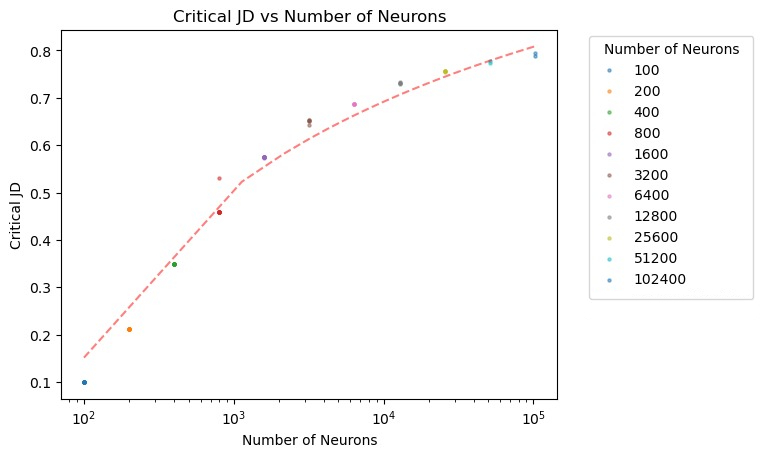
\includegraphics[width=0.8\textwidth]{Critical_JD_vs_Neurons.jpg}
  \caption{Behavior of the critical self-coupling $J^*_D$ as a function of the 
  network size $N$}
  \label{fig:critical_JD_vs_Neurons}
\end{figure}

We report the results of our numerical experiments in figure 
\ref{fig:critical_JD_vs_Neurons} where we plot the critical self-coupling
$J^*_D$ on the y-axis and the network size $N$ on the x-axis in log scale. \\
Additionally, we also plot an interpolation of the data to surmise a functional form
for the behaviour of $J^*_D$.
\vspace*{0.5em}

What is immediately noticeable is that the critical self-coupling $J^*_D$ increases 
with the network size $N$. However this growth does not appear to be linear even in 
the log scale, indicating that the relationship between the two variables has an upper
bound lower than $O\left(\log\left(N\right)\right)$.\\
Determining the exact functional form of the relationship though is not trivial, and 
further work is needed to establish a more precise relationship.

\subsection*{Convergence Times}

\begin{figure}[h!]
  \centering
  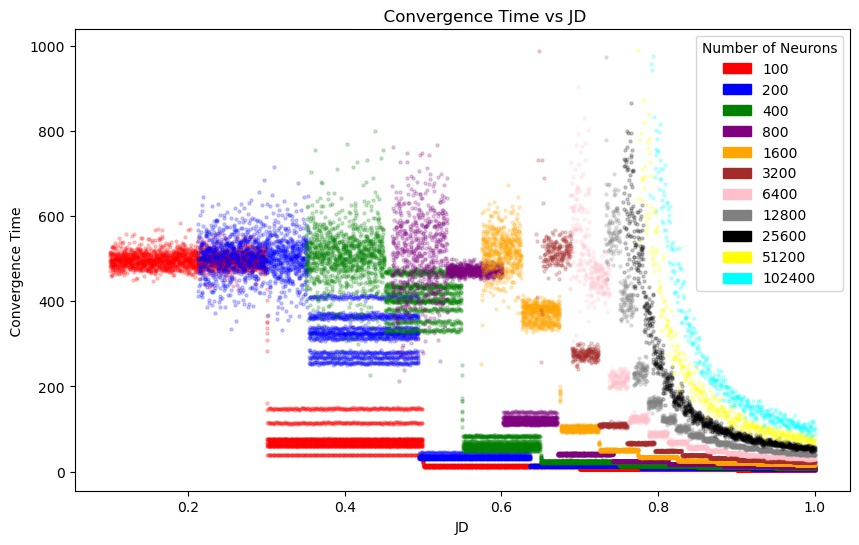
\includegraphics[width=0.8\textwidth]{Average_conv_time.jpg}
  \caption{Convergence times as a function of the self-coupling $J_D$}
  \label{fig:average_convergence_time_vs_JD}
\end{figure}

Figure~\ref{fig:average_convergence_time_vs_JD} shows the number of asynchronous update iterations required 
for full convergence as a function of the self-coupling \(J_D\), with each colour 
indicating a different network size \(N\). \\
As a confirmation of our previous results, we see that larger networks only start 
converging for larger values of \(J_D\). Indeed we notice a progressive shift to the 
right of the curves as \(N\) increases. \\
But by far the most interesting feature of this graph is the step-like plateaus: 
for smaller networks (\(N\leq 12{,}800\)), the data align on discrete horizontal 
steps each corresponding to a fixed integer number of sweeps through the neurons 
before stabilization. These plateaus arise from the granularity of the fields each 
neuron receives. In smaller networks the values that the field 
$h_i(t) = \sum_{j\neq i} J_{ij}\,s_j(t)$ can take are relatively far apart so that small 
changes in the self-coupling $J_D$ do not contribute to changing the sign in 
\ref{eq:Self_coupling_update}. \\
Indeed, as \(N\) increases, the width of each plateau in \(J_D\)-space shrinks, 
reflecting a greater sensitivity to small changes of $J_D$. Beyond roughly 
\(N=25{,}600\), the step structure becomes imperceptible and the convergence time 
\(T_c(J_D)\) is seemingly well described by a power law,
\[
  T_c(J_D)\;\propto\;(J_D - J_D^*)^{-\gamma},
\]
Though this is currently speculation and should be the object of further analyses.

\section{Stabilization through Sparse Positive Reinforcement}

We now investigate a different approach to stabilizing the dynamics of random networks.
In biological neural circuits, a small subset of synapses often exhibits 
disproportionately large, stable strengths, forming a structural backbone that 
coexists with a much larger population of weaker, plastic connections 
\cite{Scholl2020, Forsythe2013}.  
Inspired by this heterogeneity, we propose a simple stabilization scheme for 
random associative networks based on {\em sparse positive reinforcement}.
The main idea is to overlay to the random synaptc matrix \(J\) a sparse matrix 
containing positive weights, which we will refer to as the 
\emph{reinforcement matrix} $A$. \\
The network dynamics are then defined by the update rule:
\begin{equation}\label{eq:reinforcement_update}
  s_i(t+1) \;=\; \operatorname{sign}\left(\sum_{j\neq i} \left(J_{ij}+A_{ij}\right)
  \,s_j(t) \right)
\end{equation}

In the following, we will examine how the parameters \(\rho\) (sparsity level) and 
\(a\) (reinforcement strength) jointly affect the emergence of robust attractors and 
the suppression of oscillatory or chaotic regimes.

\subsection{Experimental Setup}
We implement a network of size \(N\) with:
\begin{itemize}
  \item Binary states \(s_i(t) \in \{-1,+1\}\)
  \item Random i.i.d weights 
  $J_{ij} \sim N(0,\frac{1}{\sqrt(N)}) \hspace{1em} \forall i \neq j, \hspace{1em} J_{ii} = 0 \hspace{1em} \forall i$
  \item Sparse reinforcement matrix $A$ s.t. $A_{ij} = a > 0$ non-zero for entries of 
  order $O\left(N^d\right)$ with $d \in \left(1, 2\right)$.
\end{itemize}
The update rule is given by \eqref{eq:reinforcement_update} and we once again perform 
synchronous updates.
\vspace*{0.5em}

We generate the reinforcement matrix \(A\) by first fixing the strenght $a$ and an order
for the density $O\left(N^d\right)$ and then randomly selecting a density 
\(\rho \sim N\left(N^d, \frac{1}{\sqrt{N^d}}\right)\) of non-zero entries. 
The position of the non-zero entries is chosen from a uniform distribution over the 
\(N^2\) possible positions in the matrix.

\subsection{Results}
\begin{figure}[h!]
  \centering
  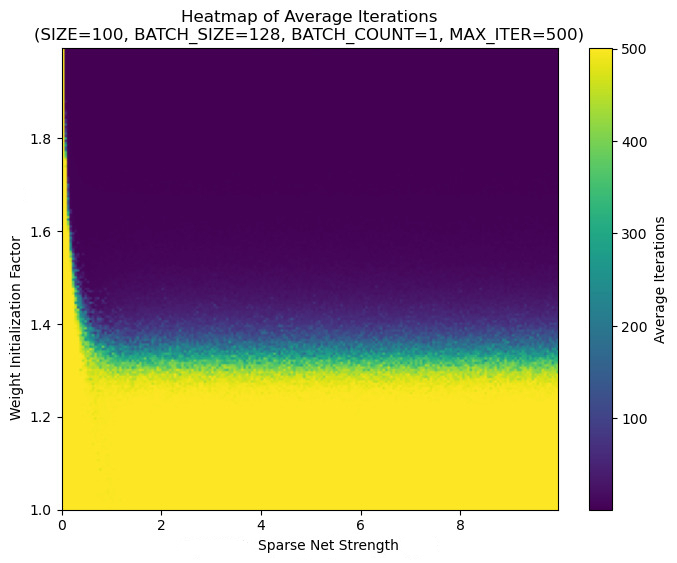
\includegraphics[width=0.4\textwidth]{100_N_avg_it.jpg}
  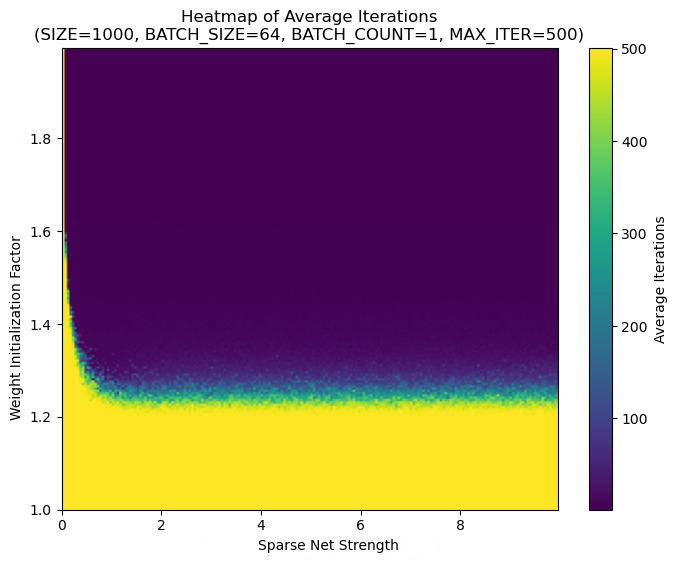
\includegraphics[width=0.4\textwidth]{1000_N_avg_it.jpg}
  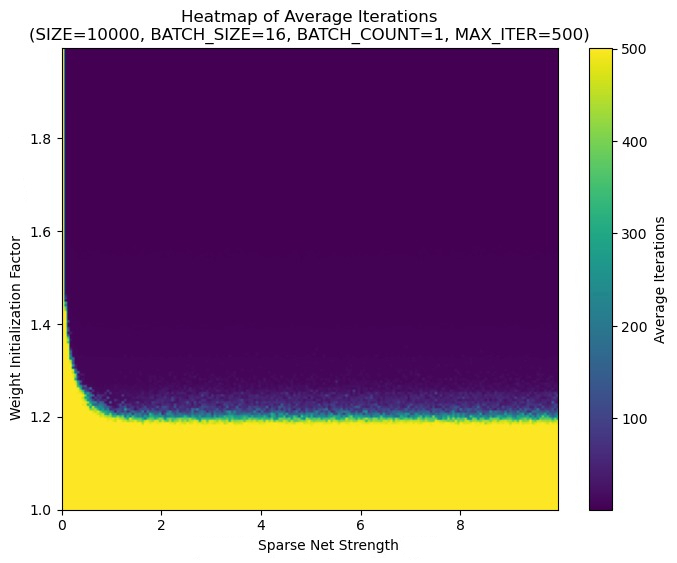
\includegraphics[width=0.4\textwidth]{10000_N_avg_it.jpg}
  \caption{Comparison of average iterations for networks of size 100, 1000, and 10000.\\
  On the x-axis we have the reinforcement strength \(a\) and on the 
  y-axis the exponential $d$ determing the order $O\left(N^d\right)$
  of the sparsity}
  \label{fig:avg_iterations_comparison}
\end{figure}

Figure \ref{fig:avg_iterations_comparison} shows the average number of iterations
taken to converge for networks of different sizes \(N\) (100, 1000, and 10000).
Since it is not possible to numerically verify whether a state does not
converge, we set a maximum number of iterations \(T_{\max} = 500\) and 
make the assumption that if the network does not converge within this time,
then it is likely to be in a chaotic regime. \\
We can distinguish three distinct dynamical regimes in the sparsity-density
plane \((d,a)\) plane, whose extents depend markedly on network size \(N\):

\begin{itemize}
  \item \emph{Chaotic regime (yellow):}  
    For sparsity exponents \(d\) in approximately the range 
    \(1.0 \lesssim d \lesssim 1.2\), no value of reinforcement 
    strength \(a\) yields convergence within the maximum iterations.  
    This disorder-dominated region persists across all \(N\), 
    indicating that below a critical sparsity order the random 
    background overwhelms the sparse foundation and the dynamics 
    remain non-attracting.

  \item \emph{Trivial regime (purple):}  
    At very high \(d\) and/or very large \(a\), almost every trial 
    converges in just a handful of iterations.  Here the sparse 
    reinforcement saturates the dynamics producing a trivial fixed 
    point that carries little information about the initial condition. 
    Further inspection indeed reveals that all states in this region 
    converge to either the all \(+1\) or all \(-1\) states, which 
    composed the only two fixed points of the dynamics.

  \item \emph{Intermediate convergence regime (green/blue):}  
    Sandwiched between the two extremes lies a band of parameter 
    combinations for which convergence occurs after a nontrivial 
    number of updates. This "sweet spot" represents the most 
    interesting operational regime, where the sparse positive backbone 
    and the random substrate jointly give rise to genuine attractor 
    dynamics.

\end{itemize}

The width of the intermediate (green/blue) band shrinks with 
increasing \(N\). Thus, although sparse positive reinforcement can 
reliably induce convergence, the "parameter margin" for nontrivial 
dynamics becomes more stringent in very large systems.
\vspace*{0.5em}

Another interesting remark is that the lower boundary of the 
chaotic region, the minimal exponent \(d_{\min}(N)\) beyond which 
convergence becomes possible, decreases as \(N\) grows. 
In other words, larger networks allow for stable dynamics even in 
progressively sparser reinforcement (\(d\)) regimes, suggesting a scaling 
law \(d_{\min}(N)\to d_\infty<2\) that merits analytic characterization.
\vspace*{0.5em} \\

Overall, these heatmaps demonstrate that sparse positive reinforcement 
can stabilize large random networks, but only within a narrowing 
window of sparsity and strength. Highlighting the need for further 
theoretical insight into the asymptotic limits of \(d\) and \(a\) 
as \(N\to\infty\).  


%--------------------------------------------------------------------------------------------------------




\chapter{Reservoir Computing}
Reservoir Computing (RC) is a computational framework particularly well-suited for 
processing temporal and sequential data. The fundamental idea behind RC is the use of a 
fixed, randomly connected recurrent neural network, known as the "reservoir", to 
project input data into a high-dimensional space. \\
Unlike traditional RNNs, the weights within the reservoir are not trained. Instead, 
only the weights of a simple linear "readout" layer connected to the reservoir's states 
are trained to perform the specific task.\\
The reservoir's complex, non-linear dynamics, driven by sequential input, create rich 
spatio-temporal patterns that capture the input's history and context. While not adapted 
to a specific task, the reservoir provides the computational preprocessing for a large
range fo possible tasks; this can then be leveraged by a simple linear readout layer to 
perform complex computations. 
Essential properties for a functional reservoir include high dimensionality, nonlinearity, 
and fading memory, which ensures sensitivity to recent inputs \cite{TANAKA2019100}.\\
In this chapter we explore the two main types of RC models: Liquid State Machines
\cite{Maass2002} and Echo State Networks \cite{Jaeger2001}.

%attach figure called 'RC_picture.png' here with a caption
\begin{figure}[h!]
    \centering
    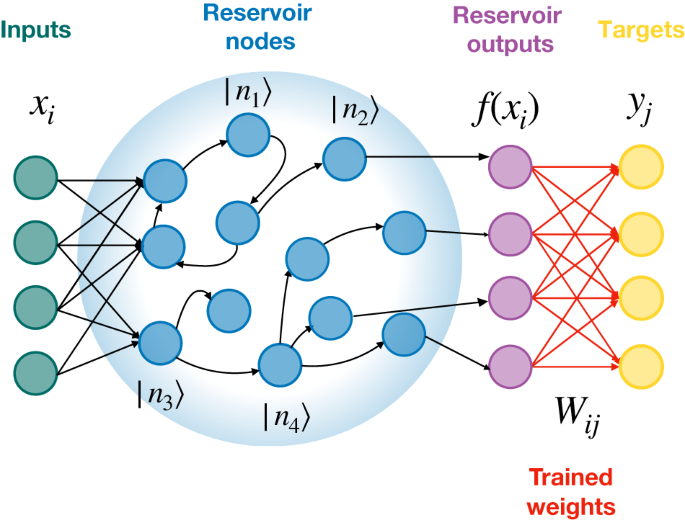
\includegraphics[width=0.8\textwidth]{RC_picture.png}
    \caption{Reservoir Computing framework. The reservoir is a fixed recurrent neural 
    network that transforms input data into a high-dimensional space. The readout layer 
    is trained to perform the specific task.}
    \label{fig:rc_framework}
\end{figure}

\section{Liquid State Machines}
Liquid State Machines (LSMs) represent a specific type of Reservoir Computing model that 
was developed with a strong emphasis on the computational capabilities of biological 
neural microcircuits within the brain \cite{Maass2002, Maass2004, Maass2011}.\\
The primary motivation behind LSMs was to create biologically relevant learning models 
using spiking neural networks (SNNs) with recurrent connectivity.
\vspace*{0.5em} \\

The computational framework of an LSM is similar to the general RC architecture, 
consisting of a reservoir (usually known as the Liquid) and a readout layer. In LSMs, 
the liquid is typically composed of excitatory and inhibitory spiking neurons. 
The input $\mathbf{u}(t)$ to the system is often encoded as a spike sequence. This input drives the 
dynamics of the liquid, typically represented as $L^M$, transforming the input into high-dimensional 
spatio-temporal patterns of neuronal activity, referred to as the reservoir/liquid state: 
$$ \mathbf{x^M}(t) := (L^M\,\mathbf{u})(t)$$ 
The output $ y(t) : = W\mathbf{x^M}(t)$ is then generated by a memory-less readout map $W$ 
that processes the reservoir state. 
A simple machine learning algorithm or a biologically plausible learning rule like the 
ones seen in section \ref{sec:learning_rules} can be used to train the readout map.

\subsection*{Biological Characteristics of the Liquid}
As birefly mentioned above, the liquid is designed to employ several biological principles,
including:
\begin{itemize}
  \item \emph{Spiking Neurons:}
    The units within the LSM reservoir are typically modeled using biologically plausible 
    spiking neuron models, such as the continuous-time leaky integrate-and-fire (LIF) 
    neuron model \cite{TANAKA2019100}. 
    This model is particularly common in theoretical neuroscience
    due its simplicity and ability to capture the essential feature of neurons (
    i.e. the integration of incoming signals and the generation of output 
    spikes when a threshold is reached). 
  \item \emph{Excitatory and Inhibitory Neurons:}
    The LSM reservoir incorporates both excitatory and inhibitory neurons, reflecting 
    the fundamental organization of biological neural networks according to Dale's law.
    Typically the ratio of excitatory to inhibitory neurons is set to 4:1, which is a
    common ratio found in biological neural networks.
  \item \emph{Biologically Constrained Connectivity}
    The topology and connectivity in the LSM reservoir are designed to adhere to 
    constraints observed in biological neural networks. For instance, the probability 
    of connection between two neurons may depend on their spatial distance 
    \cite{TANAKA2019100}.
\end{itemize}

\section{Echo State Networks}

Echo State Networks (ESNs) are another prominent type of Reservoir Computing model that 
emerged independently of Liquid State Machines (LSMs) around the same time. While both 
ESNs and LSMs share the core principles of using a fixed RNN as a 
reservoir and training only a readout layer, they differ in their specific reservoir 
implementation.
\vspace*{0.5em} \\

In contrast to the spiking neural networks typically used in LSMs which operate in 
continuous time and use spike sequences as inputs, ESNs employ reservoirs 
composed of discrete-time artificial neurons, often with sigmoid-type activation 
functions \cite{Melandri2014}. The dynamics of the neuronal states in an ESN reservoir 
are typically described as:
\begin{equation}
  \mathbf{x}(n+1) = f(W^{in}\mathbf{u}(n+1) + W\mathbf{x}(n) + W^{back}y(n))
\end{equation}
where $n$ is the (discrete) time, $x(n)$ is the state vector of the reservoir units, 
$u(n)$ is the input vector, $W^{in}$ is the input-to-reservoir weight matrix, 
$W$ is the fixed recurrent weight matrix within the reservoir, $W^{back}$ is the output-to-reservoir
weight matrix, and $f$ is the activation function. The output $y(n)$ is often a 
linear combination of the reservoir states:
\begin{equation}
  y(n) = W^{out}\mathbf{x}(n)
\end{equation}
where $W^{out}$ is the trained readout weight matrix.



%--------------------------------------------------------------------------------------------------------
%% Part II: Multi-Layer Chain Models
%--------------------------------------------------------------------------------------------------------


\part*{Part II: Multi-Layer Chain Models}
\addcontentsline{toc}{part}{Part II: Multi-Layer Chain Models}

\chapter{Introduction and Motivation}

\section{Background}
Before describing the multi-layer chain architecture, we first provide a brief overview of two key
results crucial to the development of the model.

\subsubsection*{Extension of Perceptron capacity}
The capacity of the perceptron has been extensively studied, with the seminal work by 
Cover \cite{Cover1965} establishing the conditions under which a perceptron can 
separate data.\\
In this context the measure of complexity is taken to be the maximum number of 
patterns which can be classified correctly by a perceptron. Through the use of 
Cover's Counting Theorem, it can be shown that for a perceptron with $N$ inputs, the 
probability of being able to separate $P$\footnote{
    \setstretch{1}\vspace{-0.15em}It's worth remarking that we must also assume the $P$ points to be in general position, meaning that
no subset of size less than N is linearly dependent. In practice this is a very mild condition and 
almost never happens.\vspace{-0.25em}
} with randomly assigned labels is given by:
\begin{equation}
  \mathbb{P}\left(\{ \left(\mathbf{x}_1, y_1 \right), \text{...}, 
  \left(\mathbf{x}_P, y_P \right)\} \hspace{5pt} \text{linearly separable}\right) \;=\; 
  \frac{1}{2^{P-1}} \sum_{k=0}^{N-1} \binom{P-1}{k}
\end{equation}
In the large $N$ limit, this probability approaches 1 when $P < 2N$ and approaches 0 when 
$P > 2N$. We thus conclude the capacity of the perceptron to be $2N$.
\vspace*{0.5em} \\

Surprisingly, empirical observations \cite{Student2024} have shown that passing the data through a 
Random RNN (properly constructed so as to make the dynamics stable and non-trivial) as a 
preprocessing step can increase the capacity of the perceptron. This is due to the fact that the 
network creates an internal representation of the data which better reveal the underlying structure 
of the data, thus allowing for the perceptron to separate the data more easily. In practice this 
preprocessing step is executed by setting the initial state of the RNN to be the input data, and 
then running the dynamics until convergence. \\
Through this process, the capacity of the perceptron increases from $2N \hspace{5pt} \text{to} 
\hspace{5pt} \sim 6N$.

\subsubsection*{Stabilization effects of Ferromagnetic Couplings}

\begin{figure}[h!] % Optional: put it in a figure environment for captioning and placement
    \centering
    \begin{tikzpicture}[
    circ/.style={circle, draw=black, fill=white, minimum size=1cm, thick},
    group_ellipse/.style={ellipse, draw=black, fill=gray!90, fill opacity=0.1, inner sep=-2mm, thick},
    line_style/.style={draw=red, thick},
    loop_style/.style={draw=blue!50!cyan!80!black, thick, looseness=1.5}
]

\pgfdeclarelayer{bg}    % declare background layer
\pgfsetlayers{bg,main}  % set layer order

% Left set of nodes
\node[circ] (l1) at (0,1.5) {};
\node[circ, below=0.15cm of l1] (l2) {};
\node[circ, below=0.15cm of l2] (l3) {};
\node[circ, below=0.15cm of l3] (l4) {};

% Center set of nodes
% \node[circ] (c1) at (6,1.5) {};
% \node[circ, below=0.15cm of c1] (c2) {};
% \node[circ, below=0.15cm of c2] (c3) {};
% \node[circ, below=0.15cm of c3] (c4) {};

% Right set of nodes
\node[circ] (r1) at (6,1.5) {};
\node[circ, below=0.15cm of r1] (r2) {};
\node[circ, below=0.15cm of r2] (r3) {};
\node[circ, below=0.15cm of r3] (r4) {};

% Draw ellipses around the nodes
\begin{pgfonlayer}{bg}
    \node[group_ellipse, fit=(l1) (l2) (l3) (l4), minimum width=3cm, minimum height=5cm] (ellipse_l) {};
    \node[group_ellipse, fit=(r1) (r2) (r3) (r4), minimum width=3cm, minimum height=5cm] (ellipse_r) {};
    % \node[group_ellipse, fit=(c1) (c2) (c3) (c4), minimum width=3cm, minimum height=5cm] (ellipse_c) {};
\end{pgfonlayer}

% Draw connecting loop lines between nodes with a slight bend
% \draw[line_style] (l1) to[bend left=10] (c1);
% \draw[line_style] (l2) to[bend left=10] (c2);
% \draw[line_style] (l3) to[bend left=10] (c3);
% \draw[line_style] (l4) to[bend left=10] (c4);
% \draw[line_style] (c1) to[bend left=10] (r1);
% \draw[line_style] (c2) to[bend left=10] (r2);
% \draw[line_style] (c3) to[bend left=10] (r3);
% \draw[line_style] (c4) to[bend left=10] (r4);
\draw[line_style] (l1) to[bend left=10] (r1);
\draw[line_style] (l2) to[bend left=10] (r2);
\draw[line_style] (l3) to[bend left=10] (r3);
\draw[line_style] (l4) to[bend left=10] (r4);

% Draw curved "loop" lines within left group
\draw[loop_style] (l1.west) to[bend right=30] (l2.west);
\draw[loop_style] (l2.east) to[bend left=30] (l3.east);
\draw[loop_style] (l3.west) to[bend right=30] (l4.west);
\draw[loop_style] (l1.east) to[bend left=50] (l3.east);
\draw[loop_style] (l2.east) to[bend left=50] (l4.east);
\draw[loop_style] (l1.west) to[bend right=30] (l4.west);

% Draw curved "loop" lines within center group
% \draw[loop_style] (c1.west) to[bend right=45] (c2.west);
% \draw[loop_style] (c2.east) to[bend left=45] (c3.east);
% \draw[loop_style] (c3.west) to[bend right=45] (c4.west);
% \draw[loop_style] (c1.east) to[bend left=45] (c3.east);
% \draw[loop_style] (c2.east) to[bend left=45] (c4.east);
% \draw[loop_style] (c1.west) to[bend right=30] (c4.west);

% Draw curved "loop" lines within right group
\draw[loop_style] (r1.east) to[bend left=30] (r2.east);
\draw[loop_style] (r2.west) to[bend right=30] (r3.west);
\draw[loop_style] (r3.east) to[bend left=30] (r4.east);
\draw[loop_style] (r1.west) to[bend right=50] (r3.west);
\draw[loop_style] (r2.west) to[bend right=50] (r4.west);
\draw[loop_style] (r1.east) to[bend left=30] (r4.east);

\end{tikzpicture} % This includes the TikZ/LaTeX diagram directly
    \caption{RNNs in parallel with spatial ferromagnetic connections}
    \label{fig:diagram_spatial_ferromagnetic}
\end{figure}

In section \ref{sec: sc_stabilization} we have seen that some methods that can be used to stabilize the 
dynamics of a random RNN. In particular, those methods relied on the presence of a self-coupling term
$J_D$ which acted as an inertial force that prevented each neuron from changing its state too 
frequently. \\
Borrowing a term from statistical physics, we call a "ferromagnetic" interaction a positive 
interaction between neurons which encourages them to have the same sign of activity. 
In this case, the self-coupling can be seen as a ferromagnetic connection in time between a neuron at 
time $t$ and itself at time $t-1$. \\
The positive effect that ferromagnetic coupling have on the dynamics of a random RNN is not only 
restricted to temporal connections, but can also be extended to spatial connections. Indeed research 
indicates that having multiple RNNs connected in parallel, with each neuron in each RNN not only 
being fully connected to all the other neurons in the same RNN but also being connected to other 
neurons with the same index in other RNNs, leads to a stabilization of the dynamics comparable to
that of the self-coupling term.

\section{Overview of Multi-Layer Chain Architecture}
Following the above remarks, we can construct a multi-layered architecture composed of 
multiple Random RNNs connected to each other sequentially through ferromagnetic 
connections. The idea would be to connect the input data to the first network layer, 
which would then pass along information to the next layers and so on, until the final 
layer which would then be connected to a classifier/regressor head that would output 
the prediction. We call such an architecture a Multi-Layer Chain Model (MLCM).\\
Just as Multi-Layer Perceptron networks extract more abstract features from the data 
the deeper into the network we go, the internal representation of the data in the 
MLCM is expected to become more and more instructive as we go deeper into the network.\\
Just like other architectures, MLCMs can also be trained to allow them to attune 
better to the data and specialize to the current task; crucially, this can be 
accomplished via local learning rules. Indeed, we will see in later sections that 
each neuron in each RNN layer can be thought of as a separate instance where to run 
a modified version of the perceptron learning algorithm. \\
During inference, the input data is passed to the first layer as an external input of 
a specified strength, then the dynamics of all the networks are made to run until 
convergence. The fixed point of the final layer is taken to be the internal 
representation of the data, which is then passed to the classifier head for the prediction.

\begin{figure}[h!] 
    \centering
    \begin{tikzpicture}[
    circ/.style={circle, draw=black, fill=white, minimum size=1cm, thick},
    group_ellipse/.style={ellipse, draw=black, fill=gray!90, fill opacity=0.1, inner sep=-2mm, thick},
    line_style/.style={draw=red, thick},
    input_line_style/.style={draw=red, thick},
    loop_style/.style={draw=blue!50!cyan!80!black, thick, looseness=1.5}
]

\pgfdeclarelayer{bg}    % declare background layer
\pgfsetlayers{bg,main}  % set layer order

% Input nodes
\node[circ] (i1) at (0cm,0cm) {};
\node[circ, below=0.15cm of i1] (i2) {};
\node[circ, below=0.15cm of i2] (i3) {};
\node[circ, below=0.15cm of i3] (i4) {};

% Left set of nodes
\node[circ] (l1) at (3.5cm,0cm) {};
\node[circ, below=0.15cm of l1] (l2) {};
\node[circ, below=0.15cm of l2] (l3) {};
\node[circ, below=0.15cm of l3] (l4) {};

% Center set of nodes
\node[circ] (c1) at (7cm,0cm) {};
\node[circ, below=0.15cm of c1] (c2) {};
\node[circ, below=0.15cm of c2] (c3) {};
\node[circ, below=0.15cm of c3] (c4) {};

% Right set of nodes
\node[circ] (r1) at (10.5cm,0cm) {};
\node[circ, below=0.15cm of r1] (r2) {};
\node[circ, below=0.15cm of r2] (r3) {};
\node[circ, below=0.15cm of r3] (r4) {};

% Output node
\node[circ, right=3.5cm of r2] (o1) {};
\node[circ, below=0.15cm of o1] (o2) {};

% Draw ellipses around the nodes
\begin{pgfonlayer}{bg}
    \node[group_ellipse, fit=(l1) (l2) (l3) (l4), minimum width=3cm, minimum height=5cm] (ellipse_l) {};
    \node[group_ellipse, fit=(r1) (r2) (r3) (r4), minimum width=3cm, minimum height=5cm] (ellipse_r) {};
    \node[group_ellipse, fit=(c1) (c2) (c3) (c4), minimum width=3cm, minimum height=5cm] (ellipse_c) {};
\end{pgfonlayer}

% Draw connecting loop lines between nodes with a slight bend
\draw[line_style] (l1) to[bend left=10] (c1);
\draw[line_style] (l2) to[bend left=10] (c2);
\draw[line_style] (l3) to[bend left=10] (c3);
\draw[line_style] (l4) to[bend left=10] (c4);
\draw[line_style] (c1) to[bend left=10] (r1);
\draw[line_style] (c2) to[bend left=10] (r2);
\draw[line_style] (c3) to[bend left=10] (r3);
\draw[line_style] (c4) to[bend left=10] (r4);

% Draw input lines to the left group
\draw[input_line_style] (i1) -- (l1);
\draw[input_line_style] (i2) -- (l2);
\draw[input_line_style] (i3) -- (l3);
\draw[input_line_style] (i4) -- (l4);

% Draw output line from the right group to the output node
\draw[input_line_style] (r1) -- (o1);
\draw[input_line_style] (r2) -- (o1);
\draw[input_line_style] (r3) -- (o1);
\draw[input_line_style] (r4) -- (o1);
\draw[input_line_style] (r1) -- (o2);
\draw[input_line_style] (r2) -- (o2);
\draw[input_line_style] (r3) -- (o2);
\draw[input_line_style] (r4) -- (o2);



% Draw curved "loop" lines within left group
\draw[loop_style] (l1.west) to[bend right=30] (l2.west);
\draw[loop_style] (l2.east) to[bend left=30] (l3.east);
\draw[loop_style] (l3.west) to[bend right=30] (l4.west);
\draw[loop_style] (l1.east) to[bend left=50] (l3.east);
\draw[loop_style] (l2.east) to[bend left=50] (l4.east);
\draw[loop_style] (l1.west) to[bend right=30] (l4.west);

% Draw curved "loop" lines within center group
\draw[loop_style] (c1.west) to[bend right=30] (c2.west);
\draw[loop_style] (c2.east) to[bend left=30] (c3.east);
\draw[loop_style] (c3.west) to[bend right=30] (c4.west);
\draw[loop_style] (c1.east) to[bend left=50] (c3.east);
\draw[loop_style] (c2.east) to[bend left=50] (c4.east);
\draw[loop_style] (c1.west) to[bend right=30] (c4.west);

% Draw curved "loop" lines within right group
\draw[loop_style] (r1.east) to[bend left=30] (r2.east);
\draw[loop_style] (r2.west) to[bend right=30] (r3.west);
\draw[loop_style] (r3.east) to[bend left=30] (r4.east);
\draw[loop_style] (r1.west) to[bend right=50] (r3.west);
\draw[loop_style] (r2.west) to[bend right=50] (r4.west);
\draw[loop_style] (r1.east) to[bend left=30] (r4.east);

\end{tikzpicture} %
    \caption{Diagram of MLCM architecture. The input data is passed through the network and ends up
    at the output layer, which is connected to a classifier head}
    \label{fig: MLCM}
\end{figure}

\chapter{Mathematical Formulation}

\section{Model Framework}
In the last chapter we introduced the general architecture behind MLCMs, we now 
proceed with providing a more formal definition of the model and its components. \\
Let's consider the simple case in which an input of size $N$ is passed through $L$ layers
of RNNs, each of size $N$, and then through a classifier head of size $M$. 
\vspace*{0.5em} \\

The model is composed of:
\begin{itemize}
    \itemsep-5pt
    \vspace*{-5pt}
    \item \emph{Layer Weights:} A a set of trainable randomly-initialized weights for 
    each RNN:  
    $\{ J^l \hspace{2pt} | \hspace{2pt} J^l \in \mathbb{R}^{N \times N}\}_{l=1}^{L}$
    \item \emph{Self Couplings:} A set of self-coupling weights:
    $\{ J_D \hspace{2pt} | \hspace{2pt} J_D \in \mathbb{R}\}_{l=1}^{L}$
    \item \emph{Left Ferromagnetic Couplings:} A set of ferromagnetic connections 
    connecting the previous layer $l-1$ to the current layer $l$: $ \{ \lambda_L^l 
    \hspace{2pt} | \hspace{2pt} \lambda_L^1 \in \mathbb{R}\}_{l=2}^L$
    \item \emph{Right Ferromagnetic Couplings:} A set of ferromagnetic connections
    connecting the next layer $l+1$ to the current layer $l$: $\{ \lambda_R^l
    \hspace{2pt} | \hspace{2pt} \lambda_R^L \in \mathbb{R}\}_{l=1}^{L-1}$
    \item \emph{Input Coupling:} A value determining the strength that the input data
    applies to the first layer in the form of an external field: $\lambda_{\mathrm{IN}} 
    \in \mathbb{R}$
    \item \emph{Output Coupling:} A value determining the strength that the output
    applies to the last layer in the form of an external field: $\lambda_{\mathrm{OUT}} 
    \in \mathbb{R}$
    \item \emph{Forward Output Weight:}  The weights of the perceptron predicting the 
    ouput from the final RNN layer: $W^{\mathrm{fwd}} \in \mathbb{R}^{M \times N}$.
    \item \emph{Backward Output Weight:} A weight matrix  connecting the output layer to the
    last RNN layer and determining the influence it has on it: $W^{\mathrm{back}} \in \mathbb{R}^{N \times M}$. 
\end{itemize}

We want the model to be able to take an input data vector $\mathbf{x} \in \mathbb{R}^N$ 
and pass it through the network to obtain an output vector $\mathbf{y} \in 
\mathbb{R}^M$. It stands to reason that also $\mathbf{y}$, not only $\mathbf{x}$, 
should influence the learning of the weights in the network during training. We 
implement this by projecting the output layer up to $N$ dimensions through $W^{back}$ and then allowing 
it to influence the last RNN layer in a similar way to how the input data influences 
the first RNN layer. The flow of information in MLCMs is thus bidirectional, with 
the information about the input flowing forward and the information about the output 
flowing backward simultaneously. \\
Mathematically, we update the state of a neurons in layer $l$ at time $t$ according to the
following dynamics:
\begin{equation}
    s_i^l(t+1) = 
    \begin{cases}
        \operatorname{sign}\left(\displaystyle\sum_{j \neq i} J_{ij}^l s_j^l(t) + 
        J_D\, s_i^l(t) + \lambda_{\mathrm{IN}}\, x_i + \lambda_R^l\, s_i^{l+1}(t)
        \right) & \text{if } l = 1 \\[2ex]
        \operatorname{sign}\left(\displaystyle\sum_{j \neq i} J_{ij}^l s_j^l(t) + 
        J_D\, s_i^l(t) + \lambda_L^l\, s_i^{l-1}(t) + \lambda_R^l\, s_i^{l+1}(t)
        \right) & \text{if } 1 < l < L \\[2ex]
        \operatorname{sign}\left(\displaystyle\sum_{j \neq i} J_{ij}^l s_j^l(t) + 
        J_D\, s_i^l(t) + \lambda_L^l\, s_i^{l-1}(t) + \lambda_{\mathrm{OUT}} 
        \sum_{k=1}^{M} W_{ik}^{\mathrm{back}} y_k\right) & \text{if } l = L
    \end{cases}
    \label{eq:si_update}
\end{equation}
While a prediction is made by the readout layer as:
\begin{equation}
    \hat{\mathbf{y}} = \operatorname{softmax}\left(W^{\mathrm{fwd}} \mathbf{s}^{L}_{\infty}\right)
    \label{eq:yk_update}
\end{equation}
Where $\mathbf{s}^{L}_{\infty} := \lim_{t\to\infty} \mathbf{s}^{L}(t)$ is the fixed 
point the last RNN layer converges to.

\section{Learning Dynamics}
Learning in MLCMs concerns updating the layer weights $J^l$ and the output
weights $W^{\mathrm{fwd}}$, this is due to the fact that changing the other 
parameters either affect the stability of the dynamics or the flow of information 
upon which learning is based on for the other hyperparameters. They are best thought 
of as intrinsic properties of the network and, while it is possible to have them vary 
in time, they are usually treated as constant hyperparameters.
\vspace*{0.5em} \\

At each iteration, the training protocol is divided in two steps: 
\begin{enumerate}
    \itemsep-5pt
    \vspace*{-5pt}
    \item \emph{Convergence Step:} In this step both $\mathbf{x}$ and $\mathbf{y}$ are
    passed through the network and the dynamics are left to run until convergence. As 
    long as the ferromagnetic and the self-coupling terms are set to reasonable values,
    the network dynamics are sure to converge to some fixed points 
    $\{\mathbf{s}^{1}_{\infty}, ..., \mathbf{s}^{L}_{\infty}\}$.
    
    \item \emph{Update Step:} In this step a single pass of the perceptron training
    rule updates the layer weights $J^l$, while the output weights $W^{\mathrm{fwd}}$
    are updated through the cross-entropy loss. 
\end{enumerate}

A full pseudo-code implementation of the training algorithm is present in appendix
\ref{app:mlcm_training_algorithm}. \\
\subsection{Convergence Step}
The convergence step is computed through the dynamics described in \ref{eq:si_update}. 
This step is crucial to the training of the MLCM, as it allows the network to reach an 
internal representation containing information about both the data and the label. \\
Similarly to discussions in chapter \ref{sec:random_rnn}, there are multiple ways to
update the states:
\begin{itemize}
    \itemsep-5pt
    \vspace*{-5pt}
    \item \emph{Layer-Independent Asynchronous Update:} Select a random neuron in 
    the network and update its state using the current value of $t$ for that neuron.
    Continue until all neurons in the entire MLCM have been updated. 
    \item \emph{Layer-Sequential Asynchronous Update:} Update each layer using 
    asynchronous updating, but do so going from layer 1 to layer $L$ sequentially.
    \item \emph{Layer-Sequential Synchronous Update:} Update every neuron in a layer
    at the same time, using the current value of $t$ for each neuron in that layer.
    Then proceed to the next layer and repeat until all layers have been updated.
    \item \emph{Layer-Independent Synchronous Update:} Update all neurons in the
    network at the same time, using the current value of $t$ for each neuron.
\end{itemize}
In practice, the last two methods are the most commonly used because they parallelize 
the computations through matrix multiplication and are thus much faster.
\vspace*{0.5em} \\

Usually at each iteration of training, the hidden layer states are initialized to a 
fixed initial state. This is done both to reduce the level of noise in the network as
well as to allow for batching during training, which will be discussed later.

\subsection{Update Step}
During inference, the model will not have access to the true label $\mathbf{y}$ of 
$\mathbf{x}$, thus it would be preferable for the training to be done in such a way
so that the outcome does not depend directly on the backward flow of information.
To this end, at each iteration of training we can modify the layer weights $J^l$ 
so as to try to better approximate the results obtained during the convergence step
only through the forward flow. \\
In other words, after reaching the convergence step consider a neuron $i$ in layer 
$l$: we can see it as a perceptron which as inputs has the other neurons in the same 
layer and neuron $i$ in layer $l-1$, as pre-activation signal has: $\sum_{j \neq i} 
J_{ij}^l \left(\mathbf{s}^{l}_{\infty}\right)_j + \lambda_L^l\, 
\left(\mathbf{s}^{l-1}_{\infty}\right)_i$ and as output we want to predict has 
$\left(\mathbf{s}^{l}_{\infty}\right)_i$. We can then apply the perceptron learning
rule to update the weights $J_{ij}^l$ with learning rate $\eta > 0$ as follows:
\begin{equation}
    J_{ij}^l \leftarrow J_{ij}^l + \eta \left(\left(\mathbf{s}^{l}_{\infty}\right)_i -
    \operatorname{sign}\left(\sum_{j \neq i} J_{ij}^l
    \left(\mathbf{s}^{l}_{\infty}\right)_j + \lambda_L^l\,
    \left(\mathbf{s}^{l-1}_{\infty}\right)_i\right)\right)
    \left(\mathbf{s}^{l}_{\infty}\right)_j
\end{equation}
Unlike equation \ref{eq:si_update}, this update rule actively ignores the contributions
from both itself and $\left(\mathbf{s}^{l+1}_{\infty}\right)_i$ precisely becauuse we 
want we want the model at inference to only depend on the influence of the input.

\chapter{Empirical Evaluation}

\section{Baseline Implementation with MNIST dataset}

\subsection{Experimental Setup}

\subsection{Results}

\section{Going Beyond the Perceptron}

\subsection{Experimental Setup}
\subsection{Results}

\section{Enforcing Sparsity in MLCMs}

\subsection{Experimental Setup}
\subsection{Results}

\chapter{Conclusions and Future Directions}
\section{Summary of Contributions}
\section{Limitations and Open Questions}

%--------------------
%% References and Appendices
%--------------------
\addcontentsline{toc}{chapter}{References}
\bibliographystyle{plain}
\bibliography{reference}

\appendix
\chapter{MLCM Training Algorithm}
\label{app:mlcm_training_algorithm}
We present an advanced implementation of the MLCM training algorithm, which includes 
weight decay, robustness, and initialization methods. The algorithm is designed to
train a multi-layer chain model (MLCM) using a batched input data and labels. \\
The algorithm makes use of two other algorithms: \texttt{ConversionDynamics} 
(alg. \ref{alg:conversion_dynamics}) and \texttt{UpdateSweep} (alg. \ref{alg:training_pass}).
The former is responsible for running the dynamics of the MLCM until convergence,
while the latter is responsible for updating the weights of the MLCM based on the
converged states of the MLCM and the labels. \\
\begin{algorithm}
\caption{MLCM Training Algorithm}
\label{alg:forward_mlmc}
\begin{algorithmic}[1]
\scriptsize
\Require Batched Input Data  $\mathbf{x}_{batch}$, Labels $\mathbf{y}$, 
Layer Weights $\mathbf{W}$, Self-Coupling $J_d$, Left Strength $\lambda_{L}$, 
Right Strength $\lambda_{R}$, Max Iterations $T_{max}$, Learning Rate $\eta$, 
Weight Decay $\lambda$, Robustness $\rho$, Initialization Method $init\_method$

\Statex
\Statex \textit{// Initialization Step}
\State $\mathbf{y}_{batch} \gets \mathbf{y} \cdot \mathbf{W}^{back}$
\If{$init\_method = \text{"input"}$}
    \State Initialize states $\mathbf{S}$ by repeating $\mathbf{x}_{batch}$ for $L+2$ layers
\ElsIf{$init\_method = \text{"zeros"}$}
    \State Initialize states $\mathbf{S}$ as zeros
\EndIf
\State $\mathbf{S}^0 \gets \mathbf{x}_{batch}$ \Comment{Set input as 0-th layer}
\State $\mathbf{S}^{L+1} \gets \mathbf{y}_{batch}$ \Comment{Set target's influence as 
(L+1)-th layer}

\Statex
\Statex \textit{// Convergence Step}
\State $\mathbf{S}, \mathbf{iters} \gets \text{ConversionDynamics}(\mathbf{S}, 
\mathbf{W}, J_d, \lambda_{L}, \lambda_{R}, T_{max})$
\label{line:call_conversion_dynamics}

\Statex
\If{$train$}
    \Statex \textit{// Update Step}
    \label{line:call_update_sweep}
    \State $\mathbf{W}, \mathbf{W}^{fwd} \gets \text{UpdateSweep}(\mathbf{S}, 
    \mathbf{y}, \mathbf{W}, \lambda_{L}, \lambda_{R}, \mathbf{\eta}, \mathbf{\xi}, 
    \mathbf{\rho}, \mathbf{W}^{fwd}, \eta_{ro})$
\Else
    \Statex \textit{// Output Calculation}
    \State $\mathbf{S}_{last\_rnn} \gets \mathbf{S}^L$ \Comment{States of the last RNN 
    layer}
    \State $\mathbf{logits} \gets \mathbf{W}^{fwd} \mathbf{S}^{L}$
    \State \Return $\mathbf{logits}$
\EndIf
\end{algorithmic}
\end{algorithm}


\begin{algorithm}
\caption{ConversionDynamics}
\label{alg:conversion_dynamics}
\begin{algorithmic}[1]
\scriptsize
\Require States $\mathbf{S}$, Weights $\mathbf{W}$, Self-coupling $J_d$, 
Left strength $\lambda_{L}$, Right strength $\lambda_{R}$, Max iterations $T_{max}$
\Statex
\State $t \gets 0$
\State $\mathbf{W}_{temp} \gets \mathbf{W}_{temp} + J_d \cdot \mathbf{I}$

\While{$t < T_{max}$}
    \State $\mathbf{S}_{new} \gets \mathbf{S}$
    \Statex
    \For{$l \gets 1 \text{ to } L$} \Comment{Iterate through hidden layers}
        \State $\mathbf{H}_{left} \gets \mathbf{S}_{new}^{l-1} \odot \lambda_{L}^{l-1}$
        \State $\mathbf{H}_{main} \gets \mathbf{W}_{temp}^{l-1} \mathbf{S}_{new}^l$
        \If{$train$}
            \State $\mathbf{H}_{right} \gets \mathbf{S}_{new}^{l+1} \odot \lambda_{R}^{l-1}$
        \Else
            \State $\mathbf{H}_{right} \gets \mathbf{0}$
        \EndIf
        \State $\mathbf{Field} \gets \mathbf{H}_{left} + \mathbf{H}_{main} + \mathbf{H}_{right}$
        \State $\mathbf{S}_{new}^l \gets \text{sign}(\mathbf{Field})$
    \EndFor
    \Statex
    \State $t \gets t + 1$
    \If{$\mathbf{S} = \mathbf{S}_{new}$} \Comment{Check for overall convergence}
        \State \textbf{break}
    \EndIf
    \State $\mathbf{S} \gets \mathbf{S}_{new}$
\EndWhile
\Statex
\State \Return $\mathbf{S}$
\end{algorithmic}
\end{algorithm}



\begin{algorithm}
\caption{UpdateSweep}
\label{alg:training_pass}
\begin{algorithmic}[1]
\scriptsize
\Require States $\mathbf{S}$, Target $\mathbf{y}$, Weights $\mathbf{W}$, 
Left strength $\lambda_{L}$, Right strength $\lambda_{R}$, Learning rate 
$\mathbf{\eta}$, Weight decay $\mathbf{\xi}$, Robustness $\mathbf{\rho}$, 
Read-out weights $\mathbf{W}^{fwd}$, Read-out learning rate 
$\eta_{ro}$
\Statex
\Statex \textit{// Hidden Layer Training}
\State $\mathbf{S}_{fixed} \gets \text{permute}(\mathbf{S})$ \Comment{Shape: (batch\_size, $L+2$, $N$)}

\State $\mathbf{H}_{left} \gets \mathbf{S}_{fixed}[:, 0 \text{ to } L-1] \odot \lambda_{L}$
\State $\mathbf{H}_{main} \gets \text{einsum}(\texttt{``lji,bli->blj''}, \mathbf{W}, \mathbf{S}_{fixed}[:, 1 \text{ to } L])$
\State $\mathbf{InstabilityCond} \gets ((\mathbf{H}_{left} + \mathbf{H}_{main}) \odot \mathbf{S}_{fixed}[:, 1 \text{ to } L]) \le \mathbf{\rho}$ \Comment{Added robustness}

\State $\Delta\mathbf{W} \gets \text{einsum}(\texttt{``bln,blm->lnm''}, \mathbf{S}_{fixed}[:, 1 \text{ to } L] \odot \mathbf{InstabilityCond}, \mathbf{S}_{fixed}[:, 1 \text{ to } L])$
\State $\Delta\mathbf{W} \gets \Delta\mathbf{W} \odot (\mathbf{\eta} / \text{batch\_size})$

\State $\mathbf{W} \gets \mathbf{W} \odot (1 - \mathbf{\eta} \odot \mathbf{\xi}) + \Delta\mathbf{W}$ \Comment{Weight decay is included}
\State Set diagonal of each $\mathbf{W}^l$ to $0$ \Comment{We set the self-couplings externally}

\Statex
\Statex \textit{// Read-out Layer Training through Cross-Entropy Loss}
\State $\mathbf{S}_{last\_rnn} \gets \mathbf{S}_{fixed}[:, L]$
\State $\mathbf{Logits} \gets \mathbf{W}^{fwd} \mathbf{S}^{L}$
\State $\mathbf{Predictions} \gets \text{softmax}(\mathbf{Logits})$
\State $\nabla{\mathbf{Logits}} \gets \mathbf{Predictions} - \mathbf{y}$
\State $\nabla{\mathbf{W}^{fwd}} \gets (\nabla{\mathbf{Logits}})^T \, \mathbf{S}_{last\_rnn}$
\State $\mathbf{W}^{fwd} \gets \mathbf{W}^{fwd} - \eta_{ro} \cdot \nabla{\mathbf{W}^{fwd}}$
\Statex
\State \Return $\mathbf{W}, \mathbf{W}^{fwd}$
\end{algorithmic}
\end{algorithm}

\end{document}
